%
% Main document
% ===========================================================================
% This is part of the document "Android Wear Projekt2".
% Authors: fankm1, paras1
%

% Document informations
%---------------------------------------------------------------------------
\def \module			{Modul BTI7302}					% Module name
\def \title			{Projekt 2: Android Wear}		% Title
\def \version		{X1.0}
\def \author			{Michael Fankhauser{,} Sathesh Paramasamy}
\def \logo			{BFH_Logo_C_de_fr_en_100_4CU}	% choose the correct logo in
													% the folder Bilder/BFH_Logo
%-----------------------------------------------------------------%----------

%---------------------------------------------------------------------------
\documentclass[
	a4paper,				% paper format
	10pt,					% fontsize
%	twoside,				% double-sided
	oneside,				% one-sided
	openright,				% begin new chapter on right side
	notitlepage,			% use no standard title page
	parskip=half,			% set paragraph skip to half of a line
]{scrreprt}					% KOMA-script report
%---------------------------------------------------------------------------

\raggedbottom
\KOMAoptions{cleardoublepage=plain}	% Add header and footer on blank pages


% Load Standard Packages:
%---------------------------------------------------------------------------
\usepackage[standard-baselineskips]{cmbright}

\usepackage[ngerman]{babel}		% german hyphenation
%\usepackage[latin1]{inputenc}  % Unix/Linux - load extended character set (ISO 8859-1)
%\usepackage[ansinew]{inputenc}  % Windows - load extended character set (ISO 8859-1)
\usepackage[utf8]{inputenc}    % UTF-8 - load extended charater set
\usepackage[T1]{fontenc}		% hyphenation of words with ä,ö and ü
\usepackage{textcomp}			% additional symbols
\usepackage{ae}					% better resolution of Type1-Fonts 
\usepackage{fancyhdr}			% simple manipulation of header and footer 
\usepackage{graphicx}			% integration of images
\usepackage{float}				% floating objects
\usepackage{caption}			% for captions of figures and tables
\usepackage{booktabs}			% package for nicer tables
\usepackage{tocvsec2}			% provides means of controlling the sectional numbering
\usepackage{rotating}			% rotating tables and other objects
\usepackage{pdflscape}			% change single pages landscape
\usepackage{tabularx}			% create nice tables
\usepackage{pdfpages}			% insert full pdf pages
\usepackage{nameref}			% reference by name, not by chapter number
\usepackage{dirtree}			% create directory trees
\usepackage{listings}			% include source code
\usepackage{epstopdf}			% convert eps graphics to pdf
%---------------------------------------------------------------------------

% Load Math Packages
%---------------------------------------------------------------------------
\usepackage{amsmath}			% various features to facilitate writing math formulas
\usepackage{amsthm}				% enhanced version of latex's newtheorem
\usepackage{amsfonts}			% set of miscellaneous TeX fonts that augment the standard CM
\usepackage{amssymb}			% mathematical special characters
\usepackage{exscale}			% mathematical size corresponds to textsize
%---------------------------------------------------------------------------

% Package to facilitate placement of boxes at absolute positions
%---------------------------------------------------------------------------
\usepackage[absolute]{textpos}
\setlength{\TPHorizModule}{1mm}
\setlength{\TPVertModule}{1mm}
%---------------------------------------------------------------------------					

% Definition of Colors
%---------------------------------------------------------------------------
\RequirePackage{color}							% Color (not xcolor!)
\definecolor{linkblue}{rgb}{0,0,0.8}				% Standard
\definecolor{darkblue}{rgb}{0,0.08,0.45}			% Dark blue
\definecolor{brickred}{cmyk}{0,0.89,0.94,0.28}	% Brickred
\definecolor{bfhred}{rgb}{0.776,0,0.066}			% Red
% specific colors
\definecolor{titlecolor}{rgb}{0,0.08,0.45}		% Color used for the title
%\definecolor{linkcolor}{rgb}{0,0,0.8}			% Blue for the web- and cd-version!
\definecolor{linkcolor}{rgb}{0,0,0}				% Black for the print-version!
\definecolor{code_bg}{gray}{0.8}					% Source Code Background
%---------------------------------------------------------------------------

% Hyperref Package (Create links in a pdf)
%---------------------------------------------------------------------------
\usepackage[
	pdftex,ngerman,bookmarks,plainpages=false,pdfpagelabels,
	backref = {false},					% No index backreference
	colorlinks = {true},					% Color links in a PDF
	hypertexnames = {true},				% no failures "same page(i)"
	bookmarksopen = {true},				% opens the bar on the left side
	bookmarksopenlevel = {0},			% depth of opened bookmarks
	pdftitle = {\title},					% PDF-property
	pdfauthor = {\author},				% PDF-property
	pdfsubject = {\module},				% PDF-property
	linkcolor = {linkcolor},				% Color of Links
	citecolor = {linkcolor},				% Color of Cite-Links
	urlcolor = {linkcolor},				% Color of URLs
]{hyperref}
%---------------------------------------------------------------------------

% Set up page dimension
%---------------------------------------------------------------------------
\usepackage{geometry}
\geometry{
	a4paper,
	left=28mm,
	right=15mm,
	top=30mm,
	headheight=20mm,
	headsep=10mm,
	textheight=232mm,
	footskip=15mm
}
%---------------------------------------------------------------------------

% Makeindex Package
%---------------------------------------------------------------------------
\usepackage{makeidx}				% To produce index
\makeindex						% Index-Initialisation
%---------------------------------------------------------------------------

% Glossary Package
%---------------------------------------------------------------------------
% the glossaries package uses makeindex
% if you use TeXnicCenter do the following steps:
%  - Goto "Ausgabeprofile definieren" (ctrl + F7)
%  - Select the profile "LaTeX => PDF"
%  - Add in register "Nachbearbeitung" a new "Postprozessoren" point named Glossar
%  - Select makeindex.exe in the field "Anwendung" ( ..\MiKTeX x.x\miktex\bin\makeindex.exe )
%  - Add this [ -s "%tm.ist" -t "%tm.glg" -o "%tm.gls" "%tm.glo" ] in the field "Argumente"
%
% for futher informations go to http://ewus.de/tipp-1029.html
%---------------------------------------------------------------------------
\usepackage[nonumberlist]{glossaries}
\makeglossaries

\newglossaryentry{BibTeX}{name={BibTeX},description={Programm zur Erstellung von Literaturangaben und -verzeichnissen in \TeX- oder \LaTeX-Dokumenten}}
\newglossaryentry{StwVrz}{name={Stichwortverzeichnis},description={Verzeichnis mit Stichworten aus dem Text}}



%---------------------------------------------------------------------------

% Listings Package
%---------------------------------------------------------------------------
\lstdefinestyle{CCode}{
	showspaces=false,
	showtabs=false,
	language={[ANSI]C},
	breaklines=true,
	basicstyle={\footnotesize \ttfamily},
	backgroundcolor=\color{code_bg},
	%frame=single,
	tab=\rightarrowfill,
	captionpos=b
}

\lstdefinestyle{CppCode}{
	showspaces=false,
	showtabs=false,
	language={[ISO]C++},
	breaklines=true,
	basicstyle={\footnotesize \ttfamily},
	backgroundcolor=\color{code_bg},
	%frame=single,
	tab=\rightarrowfill,
	captionpos=b
}

\lstdefinestyle{JavaCode}{
	showspaces=false,
	showtabs=false,
	language={Java},
	breaklines=true,
	basicstyle={\footnotesize \ttfamily},
	backgroundcolor=\color{code_bg},
	%frame=single,
	tab=\rightarrowfill,
	captionpos=b
}
%---------------------------------------------------------------------------

% Intro:
%---------------------------------------------------------------------------
\begin{document}					% Start Document
\settocdepth{section}			% Set depth of toc
\pagenumbering{Roman}
%---------------------------------------------------------------------------

% Set up header and footer
%---------------------------------------------------------------------------
\fancyhf{}						% clean all fields
\fancypagestyle{plain}{			% new definition of plain style

% Use this for double-sided:
%	\fancyfoot[OL,ER]{\footnotesize				% footer left part -->	version
%		V\version \\
%		\author \\
%		\today
%	}
%	\fancyfoot[OR,EL]{\footnotesize \thepage}	% footer right part --> page number
%	\fancyhead[C]{\module}						% header right part --> module name
%	\fancyhead[OR,EL]{\footnotesize \leftmark}	% footer left part -->	chapter
%	\fancyhead[OL,ER]{							% header left part --> BFH logo
%		\begin{textblock}{0}[0,0](29,9)
%			\includegraphics[scale=1.0]{Bilder/\logo}
%		\end{textblock}
%	}

% Use this for one-sided:
	\fancyfoot[L]{\footnotesize					% footer left part -->	version
		\version \\
		\author \\
		\today
	}
	\fancyfoot[R]{\footnotesize \thepage}		% footer right part --> page number
	\fancyhead[C]{\module}						% header right part --> module name
	\fancyhead[R]{\footnotesize \leftmark}		% footer left part -->	chapter
	\fancyhead[L]{								% header left part --> BFH logo
		\begin{textblock}{0}[0,0](29,9)
			\includegraphics[scale=1.0]{Bilder/BFH_Logo/\logo}
		\end{textblock}
	}
}

\renewcommand{\chaptermark}[1]{\markboth{\thechapter.  #1}{}}
\renewcommand{\headrulewidth}{0pt}				% no header stripline
\renewcommand{\footrulewidth}{0pt}				% no bottom stripline

\pagestyle{plain}
%---------------------------------------------------------------------------


% Title Page and Abstract
%---------------------------------------------------------------------------

% Project documentation template
% ===========================================================================
% This is part of the document "Android Wear".
% Authors: fankm1, paras1
%

\begin{titlepage}


% BFH-Logo absolute placed at (29,10) on A4
% Actually not a realy satisfactory solution but working.
%---------------------------------------------------------------------------
\begin{textblock}{0}[0,0](29,10)
	\includegraphics[scale=1.0]{Bilder/BFH_Logo/\logo}
\end{textblock}

% Titel / Untertitel / Autor:
%---------------------------------------------------------------------------
\begin{flushleft}

\vspace*{2cm}

\fontsize{18pt}{20pt}\selectfont
\module \\
\fontsize{12pt}{15pt}\selectfont\vspace{0.5em}

\vspace{2cm}

\fontsize{30pt}{32pt}\selectfont 
\noindent \textcolor{titlecolor}{\textbf{\title}} \\

\vspace{10cm}
\fontsize{12pt}{15pt}\selectfont
\begin{tabbing}
xxxxxxxxxxxxxxxx\=xxxxxxxxxxxxxxxxxxxxxxxx	\kill
Autor:			\> \author					\\
Datum:			\> \today					\\
Version:		\> \version					\\
\end{tabbing}
\end{flushleft}


\end{titlepage}

%
% ===========================================================================
% EOF
%

\cleardoubleemptypage
\setcounter{page}{1}
\chapter*{Vorwort}
\label{chap:vorwort}

In diesem Dokument soll, im Bereich Mobile Computing, der Wearable-Markt betrachtet werden. Dabei wird die Technologie Android Wear genauer analysiert.

\section*{Dokumentaufbau}
\label{sec:vorwort_aufbau}

Das vorliegende Dokument ist folgendermassen aufgebaut. PLATZHALTER TODO


\section*{Kontakt}
\label{sec:vorwort_kontakt}

\begin{table}[H]
	\begin{tabular}{lll} \toprule
		\textbf{Vorname Name} & \textbf{E-Mail} & \textbf{Funktion} \\ \midrule
		Dr. Andreas Danuser & andreas.danuser@bfh.ch & Auftraggeber und Betreuung\\ \midrule
		Michael Fankhauser & michael.fankhauser@students.bfh.ch & Student, Projekt 2 Realisierung \\ \midrule
		Sathesh Paramasamy & sathesh.paramasamy@students.bfh.ch & Student, Projekt 2 Realisierung \\ \bottomrule
	\end{tabular}
	\caption*{Kontaktpersonen}
	\label{tab:kontaktpersonen}
\end{table}


\section*{Versionskontrolle}
\label{sec:vorwort_versionen}

Die Versionskontrolle wir bei jeder \"Anderung der Minorversion nachgeführt.

\begin{table}[H]
	\begin{tabular}{lll} \toprule
		\textbf{Version}	& \textbf{Datum}	& \textbf{Beschreibung}											\\ \midrule
		X1.0					& 22. M\"arz 2015		& Dokumentinitialisierung										\\ \bottomrule
	\end{tabular}
	\caption*{Versionskontrolle}
	\label{tab:versionen}
\end{table}
%---------------------------------------------------------------------------

% Table of contents and listings
%---------------------------------------------------------------------------
\tableofcontents
\listoffigures
\listoftables
\cleardoublepage
%---------------------------------------------------------------------------

\pagenumbering{arabic}
\settocdepth{subsection}		% Set depth of toc

% Main part - Part I
%---------------------------------------------------------------------------
\part{Einleitung}
\label{part:teil1}
\onecolumn
\chapter{Einleitung}
\label{chap:teil1_einleitung}

Dieses Dokument soll die Möglichkeiten fur eine App-Entwicklung fur eine Smartwatch {(z.B. "LG G Watch")} und Android Wear im Rahmen einer Bachelorarbeit aufzeigen.
Damit beurteilt werden kann, ob sich diese Technologie für die Projektarbeit eignet, wird zuerst der Wearable-Markt analysiert und die bereits verfügbaren Produkte und deren Features miteinander verglichen.

% Einträge im Verzeichnis erscheinen lassen ohne hier eine Referenz einzufägen
\nocite{kopka:band1}
\nocite{raichle:bibtex_programmierung}
\nocite{MiKTeX}
\nocite{KOMA}
\nocite{TeXnicCenter}
\nocite{Marti06}
\nocite{Erbsland08}
\nocite{juergens:einfuehrung}
\nocite{juergens:fortgeschritten}

\section{Was sind Wearables}
\label{sec:teil1_was_sind_wearables}

Wearables sind kompakte Computersysteme, welche während der Anwendung am Körper des Benutzers befestigt sind.
Diese kleinen Systeme sollen den Träger beim alltäglichen Leben unterstützen.

\subsection{Beispiele}
\begin{tabular}{ll}
Armbanduhren: &	Welche ständig den Puls messen und unter Kontrolle haben \\
Brillen:	& Augmented Reality, Informationen zu Umgebung mit kleinem Display \\
Fitnesstracker: & Bewegungen registrieren und auswerten \\
Hörgeräte: & Dem Träger das Hören erleichtern
\end{tabular}

\subsection{Fachbereich Informatik}
Wearables ist ein fachübergreifendes Gebiet der Informatik, einige Fachgebiete:

- Ubiquitous Computing, die Rechnerallgegenwärtig \\
- Pervasive Computing, die Vernetzung von Alltagsgegenständen \\
- Mobile Computing, mobile Mensch zu Maschinen Kommunikation \\
- M2M, Machine-to-Machine, Informationsaustausch zwischen Zielgeräten \\
- IoT, Internet of Things, dass auf den vorhergehenden Fachbereichen basiert 

\section{Zukunft}
\label{sec:teil1_zukunft}

Wearables haben die Beziehung zwischen Konsumenten und Technologie neu definiert.
Es hilft dem Träger alltägliche Probleme zu lösen ohne damit zu interagieren.

Heute werden folgenden Aktionen aktiv mit Wearables betrieben:

- Tracken von Bewegungs- und Aktivitätsdaten \\
- Pulsmessungen \\
- Notifikationen vom Smartphone empfangen \\
- Fernsteuern von Geräten \\
- Überwachen von Schlaf \\
- Personalisierter Wecker

Schon jetzt gibt es viele Anwendungen im Bereich Wearables und es werden noch viel mehr.

In der Zukunft mögliche Funktionen:

- Authentifizierung (Auto öffnen, Türen aufschliessen, usw.) \\
- Bezahlen \\
- Lokalisierung \newline
- Lifelog (Verfolgen aller Aktivitäten) \\
- Genauere evaluieren von Bewegungs- und Aktivitätsdaten \\
- e-Health \\
- uvm. 

Es verspricht interessant zu werden und garantiert weiterhin eine schnelle technologische Entwicklung.
Viele Funktionen werden dem Träger nützen ohne das dieser eine Aktion mit dem tragbarem Geräte ausführen muss.


% Main part - Part II
%---------------------------------------------------------------------------
\part{Analyse des Wearable-Marktes}
\label{part:teil2}
\onecolumn
\chapter{Analyse des Wearable-Marktes}
\section{Überblick}
	\begin{itemize}
		\item verschiedene OS
			\begin{itemize}
				\item Android Wear
				\item WebOS
			\end{itemize}
		\item Vor-/Nachteile OS'
			\begin{itemize}
				\item z.B. sowohl mit AndroidWear als auch mit iOS nutzbar
			\end{itemize}
	\end{itemize}

\subsection{Marktanteile Anbieter}
\begin{figure}[h!]
	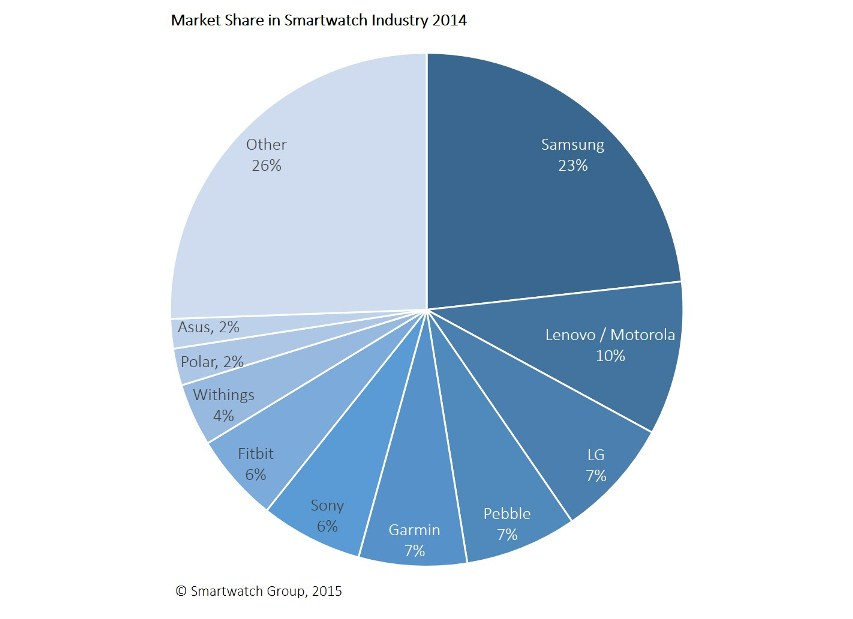
\includegraphics{Bilder/Market_Share_Smartwatch_Companies_2014}
	%\captionsetup{width=0.6\textwidth}	
	\caption[Marktanteile Smartwatch-Anbieter 2014]{Marktanteile Smartwatch-Anbieter 2014\\\hspace{\textwidth}(Quelle: http://www.smartwatchgroup.com)}
\end{figure}

\section{Prognose}
\section{Fitnesstracker}
\subsection{Definition}
Ein Fitness Tracker, auch Fitness-Armband, Smart Band oder Activity Tracker, ist ein Gerät oder eine Applikation zur Aufzeichnung und Versendung Fitness-relevanter Daten wie etwa Laufstrecken, Kalorienverbrauch und in manchen Fällen auch Herzschlagfrequenz oder Schlafqualität. Die Bezeichnung wird hauptsächlich für am Körper tragbare elektronische Überwachungsgeräte verwendet, welche, in vielen Fällen drahtlos, mit einem Computer oder Smartphone für die Datenerfassung über einen längeren Zeitraum synchronisiert werden. Abgesehen von diesen tragbaren Geräten, gibt es auch vergleichbare Applikationen für Smartphones und Facebook.\footnote{Quelle: \url{http://de.wikipedia.org/wiki/Activity\_Tracker}, Stand: 25.03.2015}

\subsection{Aktuelle Beispielgeräte}
\begin{longtable}{p{4cm}p{4cm}p{4cm}p{4cm}}

	% 1. line
	  \rule{0pt}{120pt}
	  \rotatebox{90}{Samsumg Gear Fit} 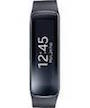
\includegraphics{Bilder/FitnessTracker/samsung_gear_fit}
	& \rotatebox{90}{Garmin Vivosmart} 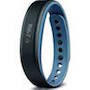
\includegraphics{Bilder/FitnessTracker/garmin_vivosmart}
	& \rotatebox{90}{Fitbit Charge HR} 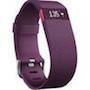
\includegraphics{Bilder/FitnessTracker/fitbit_charge_hr}
	& \rotatebox{90}{LG Lifeband Touch} 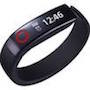
\includegraphics{Bilder/FitnessTracker/lg_lifeband_touch}\\
    % 2. line
      \rule{0pt}{120pt}
      \rotatebox{90}{Runtastic Orbit} 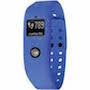
\includegraphics{Bilder/FitnessTracker/runtastic_orbit}
	& \rotatebox{90}{Withings Activité} 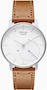
\includegraphics{Bilder/FitnessTracker/withings_activite}
	& \rotatebox{90}{Huawei TalkBand} 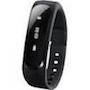
\includegraphics{Bilder/FitnessTracker/huawei_talkband}
	& \rotatebox{90}{Sony SmartBand Talk} 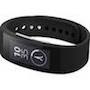
\includegraphics{Bilder/FitnessTracker/sony_smartband_talk}\\
\end{longtable}

\newpage

\section{Smartwatches}
\subsection{Definition}
Eine Smartwatch (englisch für schlaue Uhr) ist eine Armbanduhr, die zusätzlich über Sensoren, Aktuatoren (z. B. Vibrationsmotor) sowie zusätzliche Computerfunktionalität und -konnektivität verfügt. Aktuelle Smartwatches können neben der Uhrzeit weitere Informationen darstellen und lassen sich meist über zusätzliche Programme (sogenannte Apps) vom Anwender individuell mit neuen Funktionen aufrüsten.\footnote{Quelle: \url{http://de.wikipedia.org/wiki/Smartwatch}, Stand: 25.03.2015}
\newpage

% --- Vergleich Features ---
\begin{landscape}
\subsubsection{Vergleich Features}
\renewcommand{\arraystretch}{1.5}
% --- Vergleich Features, Teil 1 ---
\begin{longtable}{p{2.8cm}p{3.5cm}p{3.5cm}p{3.5cm}p{3.5cm}p{3.5cm}}

	% Header
	& \rotatebox{90}{LG G Watch} 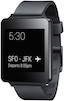
\includegraphics{Bilder/SmartWatch/lg_g_watch}
	& \rotatebox{90}{LG G Watch R} 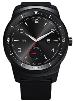
\includegraphics{Bilder/SmartWatch/lg_g_watch_r}
	& \rotatebox{90}{LG Watch Urbane LTE} 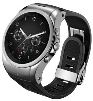
\includegraphics{Bilder/SmartWatch/lg_watch_urbane_lte}
	& \rotatebox{90}{Motorola Moto 360} 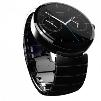
\includegraphics{Bilder/SmartWatch/moto_360}
	& \rotatebox{90}{Apple Watch} 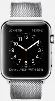
\includegraphics{Bilder/SmartWatch/apple_watch}\\
	\hline
	\endfirsthead
	
	\multicolumn{3}{l}{Fortsetzung} \\
	& {LG G Watch}
	& {LG G Watch R}
	& {LG Watch Urbane LTE}
	& {Motorola Moto 360}
	& {Apple Watch} \\
	\hline
	\endhead

	% Content
	Display
		& 1.65 Zoll \newline
			280x280px (204ppi) \newline
			IPS
		& 1.3 Zoll \newline
			320x320px (245ppi) \newline
			P-OLED
		& 1.3 Zoll \newline
			320x320px (245ppi) \newline
			P-OLED
		& 1.56 Zoll \newline
			320x290 (205ppi) \newline
			IPS
		& 1.32 Zoll \newline
			272x340 \\
	Prozessor
		& 1,2-GHz \newline Snapdragon 400
		& 1,2-GHz \newline Snapdragon 400
		& 1,2-GHz \newline Snapdragon 400
		& 1-GHz \newline Texas Instrument\newline OMAP 3
		& Apple S1 (SIP)\newline System in a package \\
	RAM
		& 512 MB
		& 512 MB
		& 1 GB
		& 512 MB
		& SIP\\
	interner Speicher
		& 4 GB
		& 4 GB
		& 4 GB
		& 4 GB
		& 8 GB \\
	Akku
		& 400 mAh
		& 410 mAh
		& 700 mAh
		& 320 mAh
		& ab 205 mAh\\
	Betriebssystem
		& Android Wear
		& Android Wear
		& LG Wear Platform \newline (ehem. HP WebOS)
		& Android Wear
		& Watch OS \\
	Kompatibilität
		& Android 4.3+
		& Android 4.3+
		& Autonom
		& Android 4.3+
		& iOS 8+\\
	Netzwerk
		& -
		& -
		& LTE
		& - 
		& -\\
	Verbindung
		& BLE 4.0
		& BLE 4.0
		& BLE 4.0 \newline
			Wifi 802.11 b/g/n \newline
			NFC
		& BLE 4.0 \newline
			WiFi
		& BLE 4.0 \newline
			WiFi 802.11 b/g/n \newline
			NFC \\
	Schnittstellen
		& Mikrofon
		& Mikrofon
		& Mikrofon \newline
			Lautsprecher
		& Mikrofon
		& Mikrofon \newline
			Lautsprecher \\
	Sensoren
		& Beschleunigungssensor \newline
			Gyroskop \newline
			Kompass \newline
			Schrittzähler
		& Herzfrequenz \newline
        		Beschleunigungssensor \newline
			Gyroskop \newline
			Kompass \newline
			Schrittzähler
		& Herzfrequenz \newline
        		Beschleunigungssensor \newline
			Gyroskop \newline
			Kompass \newline
			Schrittzähler \newline
			Luftdrucksensor
		& Herzfrequenz \newline
		    Beschleunigungssensor \newline
			Gyroskop \newline
			Kompass \newline
			Schrittzähler
		& Beschleunigung \newline
			GPS \newline
			Gyrometer \newline
			Herzfrequenz \newline
			Kompass \newline
			Multi \& ForceTouch \newline
			Schrittzähler \\
	Sonstiges
		& IP67 \newline
			Always-On Display
		& IP67
		& IP67
		& IP67
		& spritzwassergeschützt \\
	Abmessung
		& 37.9 x 45.6 x 9.95 mm
		& 46.4 x 53.6 x 11.1 mm
		& 46 x 52 x 10.9 mm
		& 46 x 46 x 11.5 mm
		& 38.6 x 33.3 x 10.5 mm \newline
		42 x 35.9 x 10.5 mm\\
	Gewicht
		& 63g
		& 62g
		& 45 - 115g
		& 49 - 124g
		& ab 73g\\ 
	Markteinführung
		& Jun 2014
		& Nov 2014
		& na 
		& Sep 2014
		& Apr 2015\\
	Preis\footnote{Preise von digitec.ch (günstigstes Modell), Stand: 17.03.2015 oder neuer}
		& CHF 99.00
		& CHF 199.00
		& na
		& CHF 199.00
		& ab CHF 389.00 \\
	\hline
	\caption{Vergleich Features von Smartwatches, Teil 1} \\
\end{longtable}
\newpage

% --- Vergleich Features, Teil 2 ---
\begin{longtable}{p{2.8cm}p{3.5cm}p{3.5cm}p{3.5cm}p{3.5cm}p{3.5cm}}

	% Header
	& \rotatebox{90}{Huawei Watch} 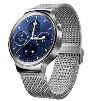
\includegraphics{Bilder/SmartWatch/huawei_watch}
	& \rotatebox{90}{Sony SmartWatch 3} 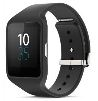
\includegraphics{Bilder/SmartWatch/sony_smartwatch_3}
	& \rotatebox{90}{Samsung Gear S} 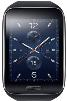
\includegraphics{Bilder/SmartWatch/samsung_gear_s}
	& \rotatebox{90}{Samsung Gear Live} 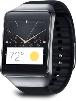
\includegraphics{Bilder/SmartWatch/samsung_gear_live}
	& \rotatebox{90}{Asus ZenWatch} 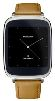
\includegraphics{Bilder/SmartWatch/asus_zen_watch} \\
	\hline
	\endfirsthead
	
	\multicolumn{3}{l}{Fortsetzung} \\
	& {Huawei Watch}
	& {Sony SmartWatch 3}
	& {Samsung Gear S}
	& {Samsung Gear Live}
	& {Asus ZenWatch} \\
	\hline
	\endhead	

	% Content
	Display
		& 1.4 Zoll \newline
			400x400 (286ppi) \newline
			AMOLED
		& 1.6 Zoll \newline
			320x320px
		& 2 Zoll \newline
			480x360px (300ppi) \newline
			Super AMOLED
		& 1.63 Zoll \newline
			320x320px (278ppi) \newline
			Super AMOLED
		& \newline
			320x320px (278ppi) \newline
			AMOLED \\
	Prozessor
		& 1.2 GHz \newline
			Snapdragon 400
		& na
		& na
		& na
		& \\
	RAM
		& 512 MB
		& 512 MB
		& 512 MB
		&
		& 512 MB\\
	interner Speicher
		& 4 GB
		& 4 GB
		& 4 GB
		& 4 GB
		& 4 GB\\
	Akku
		& 300 mAh
		& 420 mAh 
		& 300 mAh
		& 300 mAh
		& 369 mAh\\
	Betriebssystem
		& Android Wear
		& Android Wear
		& Tizen 
		& Android Wear
		& Android Wear \\
	Kompatibilität
		& Android 4.3+
		& Android 4.3+
		& Android 4.3+
		& Android 4.3+
		& Android 4.3+ \\
	Netzwerk
		& -
		& -
		& 3G
		& -
		& -\\
	Verbindung
		& BLE 4.0
		& BLE 4.0 \newline
			NFC
		& BLE 4.0
		& BLE 4.0
		& BLE 4.0\\
	Schnittstellen
		& Mikrofon
		& Mikrofon \newline
			Lautsprecher
		& Mikrofon
		& Mikrofon
		& Mikrofon \\
	Sensoren
		& Beschleunigungssensor \newline
			Gyrometer \newline
			Herzfrequenz \newline
			Schrittzähler
		& Beschleunigungssensor \newline
			Gyrometer \newline
			Kompass \newline
			GPS
		& Beschleunigungssensor \newline
			GPS \newline
			Gyrometer \newline
			Helligkeitssensor\newline			
			(Multi-)Touch
		& Beschleunigungssensor \newline
			Gyrometer \newline
			Herzfrequenz \newline
			(Multi-)Touch \newline
			Schrittzähler 
		& Beschleunigungssensor \newline
			Gyrometer \newline
			Kompass \newline
			GPS\\
	Sonstiges
		& IP67
		& IP68
		& IP67 \newline
			Kopfhörerbuchse
		&
		& IP55\\
	Abmessung
	    & 42 x 42 x 11.3 mm
		& 46.4 x 53.6 x 11.1 mm
		& 46 x 52 x 10.9 mm
		& 46 x 46 x 11.5 mm
		& 42 x 35.9 x 10.5 mm\\
	Gewicht
		& na
		& 45g
		& na
		& 59g
		& 75g\\ 
	Markteinführung
		\\
	Preis\footnote{Preise von digitec.ch (günstigstes Modell), Stand: 17.03.2015 oder neuer}
		& CHF 349.00	
		& CHF 229.00
		& CHF 329.00
		& -
		& CHF 249.00\\
	\hline
	\caption{Vergleich Features von Smartwatches, Teil 2} \\
	
\end{longtable}
\end{landscape}

\section{Andere Wearables}
http://www.digitsole.com/

\section{Verfügbare Apps/Frameworks}
http://die-smartwatch.de/android-wear-apps\#musthave\\
http://die-smartwatch.de/2015/03/15/umwelt-computer-per-android-wear-und-pebble-sperren.html\\
http://www.kiwimotion.io/
%-Included in 01_Analyse_WearableMarkt: 03_Teil_2/02_Feature_Tabelle

% Main part - Part III
%---------------------------------------------------------------------------
\part{Evaluation von Applikationen}
\label{part:teil3}
\onecolumn
\chapter{Evaluation von Applikationen}
\section{Brainstorming Ergebnisse}
\subsection{Überwachung}
\textbf{Gesundheit:}\\
- Sturz erkennen {(z.B Alarmauslösung, wenn nicht innerhalb von ca. 30s Bestätigung erfolgt)}\\
- Puls überwachen

\textbf{Alarming:}\\
- Spital: Pflegeperson erhält {(Patienten-)}Alarm auf Smartwatch

\textbf{Sport:}\\
- Aufzeichnung Bewegungen\\
- Messung der Körper-Belastung {(Beschleunigung)}

\subsection{RemoteControl}
- Smart  Home\\
- Lichtsteuerung\\
- TV/Media-Geräte\\
- Funktionen für blinde Leute

\subsection{Proximity}
- Reminder{,} wenn ausserhalb Reichweite Handy {(z.B. Handy zu Hause vergessen)}\\
- Leute in der Nähe\\
- Umgebungsradar

\subsection{Navigation}
- Indoornavigation\\
- Mitarbeiter Positionierung

\subsection{Authentication}
- Entsperren von Türen/Accounts\\
- Zugangskontrolle in Büros\\
- Zeiterfassung von Mitarbeitern

\subsection{Payment}
- Zahlungen durchführen {(Kreditkarte/Konto/Paypal)}

\newpage

% Attachment:
%---------------------------------------------------------------------------
\part{Anhang}
\label{part:anhang}
\onecolumn
\appendix
\settocdepth{section}
\chapter{Beliebiger Anhang}
\label{chap:bel_anhang}

Hier ist unser Anhang

\chapter{Weiterer Anhang}
\label{chap:anhang_B}

\section{Test 1}

Spezifischer Anhang

\subsection{Umfeld}

Spezifischer Anhang 2

%---------------------------------------------------------------------------

% Glossary
%---------------------------------------------------------------------------
\cleardoublepage
\phantomsection 
\addcontentsline{toc}{chapter}{Glossar}
\renewcommand{\glossaryname}{Glossar}
\printglossary
%---------------------------------------------------------------------------

% Bibliography
%---------------------------------------------------------------------------
\cleardoublepage
\phantomsection 
\addcontentsline{toc}{chapter}{Literaturverzeichnis}
\bibliographystyle{IEEEtranS}
\bibliography{Datenbanken/bibliography}{}
%---------------------------------------------------------------------------

% Index
%---------------------------------------------------------------------------
%\cleardoublepage
%\phantomsection 
%\addcontentsline{toc}{chapter}{Stichwortverzeichnis}
%\renewcommand{\indexname}{Stichwortverzeichnis}
%\printindex
%---------------------------------------------------------------------------

%---------------------------------------------------------------------------
\end{document}
